\documentclass{article}\usepackage[]{graphicx}\usepackage[]{color}

\title{Needs a title}
\author{Sang Woo Park, Benjamin M Bolker}

\usepackage{tabularx}

\usepackage{amsmath}
\usepackage{natbib}
\usepackage{hyperref}
\bibliographystyle{chicago}
\date{\today}

\usepackage{bm}

\usepackage{afterpage}
\usepackage{pdflscape}

\newcommand{\etal}{\textit{et al.}}

\newcommand{\comment}[3]{\textcolor{#1}{\textbf{[#2: }\textit{#3}\textbf{]}}}
\newcommand{\bmb}[1]{\comment{cyan}{BMB}{#1}}
\newcommand{\swp}[1]{\comment{magenta}{SWP}{#1}}

\newcommand{\fref}[1]{Fig.~\ref{fig:#1}}
\IfFileExists{upquote.sty}{\usepackage{upquote}}{}
\begin{document}

\maketitle

\section{Introduction}

The evolution of sexual reproduction presents a continuing question \citep{otto2009evolutionary}.
Despite being the dominant mode of reproduction \citep{vrijenhoek1998animal}, \bmb{among?} sexual reproduction entails numerous costs \citep{lehtonen2012many}.
The most commonly mentioned is the cost of producing males \citep{smith1978evolution}.
As males cannot produce offspring, sexual lineages is expected to be outgrown by their asexual counterpart that can grow as twice as fast (assuming that the sexual population produces 50\% male and 50\% female).
This infamous \emph{two-fold cost of sex} \citep{smith1978evolution} relies on the assumption that everything else is equal.
Then, what else is not equal and drives the sex to persist?

One explanation for the persistence of sexual reproduction is the Red Queen Hypothesis \citep{bell1982masterpiece}.
The Red Queen Hypothesis suggests that sexually reproducing hosts overcome the cost of sex under strong parasite selection by producing genetically diverse offspring that are resistant to infection \citep{jbs1949disease, jaenike1978hypothesis, hamilton1980sex}.
Host-parasite coevolution constantly creates selective advantage for rare genotypes, creating oscillation in genotypic frequencies, and allows for sexual reproduction to persist in the host population \citep{clarke1976ecological, hamilton1980sex}.

Much of the theoretical work has focused on determining conditions under which parasite selection can maintain sexual reproduction in the host population.
\cite{may1983epidemiology} first noted that parasites must be extremely virulent to maintain sexual reproduction but later studies showed that sexual and asexual hosts can coexist even at intermediate virulence \citep{howard1994parasitism}.
\cite{agrawal2002infection} compared a wide range of infection genetics that determine parasite resistance and the dynamics that arise from different genetic architecture.
\cite{ashby2015diversity} showed that host genetic diversity also plays an important role in determining the strength of selection for sexual reproduction.

Some theoretical studies have departed from the classical population genetics framework to study effects of ecological and epidemiological structures on the Red Queen dynamics.
Number of studies showed that incorporating ecological and epidemiological details can assist in supporting sexual reproduction in the host population \citep{galvani2001antigenic, galvani2003maintenance, lively2009maintenance, lively2010epidemiological}.
In contrary to these findings, \cite{macpherson2017joint} showed that Red Queen dynamics (i.e., cycles in allele frequencies) fail to persist when explicit epidemiological structure is taken into account with coevolutionary dynamics.

On the other hand, empirical studies have mostly focused on confirming predictions that stem from the Red Queen Hypothesis.
Typical among them are local adaptation, time-lagged selection, and association between parasite prevalence and host reproductive mode (see \cite{tobler2008expanding} and \cite{vergara2014infection} for reviews).
A key example is the snail population in New Zealand that serve as an intermediate hosts for trematodes [CITE].
Through several decades of work, Lively \etal\ demonstrated that the population satisfies necessary conditions for the host-parasite coevolutionary dynamics and provide support for the hypothesis \citep{lively1987evidence, lively1989adaptation, dybdahl1995host, dybdahl1998host, jokela2009maintenance, vergara2014infection, gibson2016within}.
While many studies provide only indirect evidence, 
recent studies show that more direct evidence can be achieved using experimental systems \citep{auld2016sex, slowinski2016coevolutionary}.

Even though the Red Queen Hypothesis has gained some support both theoretically and empirically, there still remains a gap between theory and data.
Many models for Red Queen Hypothesis rely on simplifying assumptions that are not applicable to natural populations and make predictions based on assumed parameters.
In particular, none of the Red Queen models reviewed by \cite{ashby2015diversity} use statistical tools to relate model to data.
However, there are exceptions:
\cite{lively1992parthenogenesis} postulated that infection prevalence should be positively correlated with frequency of sexual hosts and later formalized the idea with a mathematical model \citep{lively2001trematode}.
The prediction has since been confirmed by many empirical studies, most of which are based on the snail-trematode system \citep{lively2002temporal, kumpulainen2004parasites, vergara2013geographic, mckone2016fine, gibson2016within}.
Surprisingly such correlation was not observed in a different snail-trematode system \citep{dagan2013clonal}.
\bmb{A little more on qualitative requirements?}
\swp{What do you mean?}

Here, we try to bridge the gap between theory and data further.
We extend the model used by \cite{lively2010epidemiological} to account for demographic stochasticity and simple population structure.
Then, we fit the model to observational data from \cite{dagan2013clonal, mckone2016fine, vergara2014infection} using Approximate Bayesian Computation (ABC) to estimate biologically relevant parameters.
Using estimated parameters, we assess model fits and perform a power analysis to test the prediction that infection prevalence is positively correlated with frequency of sexual reproduction \cite{lively2001trematode}.
\bmb{More on power analysis}

\section{Methods}

\subsection{Data}

We consider observational data from two snail-trematode populations in New Zealand \citep{vergara2014infection, mckone2016fine} and a similar snail-trematode population in Israel \citep{dagan2013clonal}. 
The snail-trematode system has been extensively studied under the context of the Red Queen Hypothesis so we expect a simple Red Queen model to fit reasonably well.
Data collected by \cite{dagan2013clonal} and \cite{vergara2014infection} were obtained from their Dryad repositories \citep{dryad_f5t56, dryad_29nk3_2} and data collected by \cite{mckone2016fine} was extracted from their figure.

\subsection{Model}

\swp{TODO: read Lively 2018}
We model obligately sexual hosts competing with obligately asexual hosts in a meta-population by extending the model introduced by \cite{lively2010epidemiological}.
The model is a discrete time susceptible-infected (SI) model with natural mortality and virulence (defined as reduction in offspring production among infected hosts).
It is a suitable canditate model for this study as it captures essential structures that are present in basic epidemiological and population genetics models and is general enough to be applied to broad range of natural systems.
We do not consider mechanistic details of the snail-trematode system such as life history of trematodes \citep{vergara2014infection}.
We incorporate population structure and allow for mixing between populations.
Each population can be equivalently considered as a sampling site in the observed populations.

All hosts are assumed to be diploids with two biallelic loci, and parasites are assumed to be haploids.
Let $S_{ij}^k(t)$ and $A_{ij}^k(t)$ be the number of sexual and asexual hosts with genotype $ij$ from population $k$ at generation $t$. 
For simplicity, we drop the superscript representing population and write $S_{ij}(t)$ and $A_{ij}(t)$;
every population is governed by the same set of equations unless noted otherwise (e.g., when we account for interaction between populations).
Following \cite{lively2010epidemiological}, the expected amount of genotypic contribution (before recombination or outcrossing) by sexual hosts is given by
\begin{equation}
S_{ij}' = c_b (1-s) \left(W_U S_{ij,U} (t) + W_I S_{ij,I} (t)\right),
\end{equation}
where $s$ is the proportion of males produced by sexual hosts, and $S_{ij, U}$ and $S_{ij,I}$ are the number of uninfected and infected sexual hosts in a population.
$W_U$ and $W_I$ represent their corresponding fitnesses where virulence is defined as $V = 1-W_I/W_U$.
We allow for cost of sex to vary by multiplying a scale parameter, $c_b$, to the growth term, where $2/c_b$ corresponds to a two fold cost of sex \citep{ashby2015diversity}.
Recombination and outcrossing are modeled after incorporating genotypic contributions from other populations.

We define
$$
W_U = \frac{b_U}{1 + a_U N(t)}, W_I = \frac{b_I}{1 + a_I N(t)}
$$
where $b_U$ and $b_I$ are number of offspring produced by uninfected and infected hosts, respectively, and $a_U$ and $a_I$ determine their corresponding density dependent effects \citep{lively2010epidemiological, smith1973stability}.
For simplicity, we assume that $a_U = a_I$ so that virulence can be defined strictly in terms of decrease in offspring production and is constant for any density: $V = 1- b_I/b_U$.
\bmb{more specific}
\swp{Lively doesn't say much beyond this... I think it's OK?}

Asexual hosts are assumed to be strictly clonal. Then, the expected amount of genotypic contribution by asexual hosts is given by
\begin{equation}
A_{ij}' = W_U A_{ij,U} (t) + W_I A_{ij,I} (t),
\end{equation}
where $A_{ij, U}$ and $A_{ij,I}$ are the number of uninfected and infected asexual hosts in a population.

We assume that proportion $\epsilon_{\textrm{\tiny mix}}$ of a population mix with other populations.
Then, the expected number of offspring in the next generation (accounting for contributions from all populations) is given by
\begin{equation}
\begin{aligned}
\mathrm{E}\left(S_{ij}^k(t+1)\right) &= f_{\textrm{\tiny sex}}\left((1 - \epsilon_{\textrm{\tiny mix}}) \left(S_{ij}^k\right)' + \frac{\epsilon_{\textrm{\tiny mix}}}{n_{\textrm{\tiny pop}}-1} \sum_{h \neq k} \left(S_{ij}^h\right)'\right),\\
\mathrm{E}\left(A_{ij}^k(t+1)\right) &= (1 - \epsilon_{\textrm{\tiny mix}}) \left(A_{ij}^k\right)' + \frac{\epsilon_{\textrm{\tiny mix}}}{n_{\textrm{\tiny pop}}-1} \sum_{h \neq k} \left(A_{ij}^h\right)',\\
\end{aligned}
\end{equation}
where $f_{\textrm{\tiny sex}}(x)$ is the function that models sexual reproduction, including recombination probability $r_{\textrm{\tiny host}}$ and outcrossing, and $n_{\textrm{\tiny pop}}$ is the number of populations modeled.
Then, the total number of sexual and asexual hosts in the next generation given by Poisson random variables with mean specified previously. We also allow for stochastic migration to avoid fixation:
\begin{equation}
\begin{aligned}
S_{ij}^k(t+1) &\sim \mathrm{Poisson}\left(\lambda=\mathrm{E}\left(S_{ij}^k(t+1)\right)\right) + \mathrm{Bernoulli}\left(p=p_{ij,\textrm{\tiny sex}}\right),\\
A_{ij}^k(t+1) &\sim \mathrm{Poisson}\left(\lambda=\mathrm{E}\left(A_{ij}^k(t+1)\right)\right) + \mathrm{Bernoulli}\left(p=p_{ij, \textrm{\tiny asex}}\right),
\end{aligned}
\end{equation}
where $p_{ij,\textrm{\tiny sex}}$ and $p_{ij, \textrm{\tiny asex}}$ are the probabilities of a sexual and an asexual host with genotype $ij$ entering a popualation.

\bmb{No epistasis?}
\swp{Is this clearer?}
Infection is modeled using the matching alleles model \citep{otto1998evolution}.
We assume that snails are equally susceptible to parasites that match either haplotype.
However, parasites must carry same alleles in both loci in order to match a host haplotype.
The total number of infected hosts that carry parasite with genotype $i$ at generation $t$ is given by:
\begin{equation}
I_{i}(t) = \sum_{p} 2^{\delta_{ij}} \left( S_{ij,i,I}(t) + A_{ij,i,I}(t)\right),
\end{equation}
where a $\delta_{ij}$ is Kronecker delta.
$\delta_{ij}$ equals 1 when $i = j$ and 0 otherwise.
$S_{ij,i,I}(t)$ and $A_{ij,i,I}(t)$ represent the expected numbers of sexual and asexual hosts that have genotype $ij$ and are infected with genotype $i$ parasite. 
Following \cite{ashby2015diversity}, we assume that mutation can occur in one locus with probability $r_{\textrm{\tiny parasite}}$. 
Mutation is modeled using a deterministic process, as we introduce stochasticity during the actual infection process.
We also allow for stochastic external migration of an infected host carrying parasite $i$ with probability $p_{i, \textrm{\tiny parasite}}$ to avoid fixation.

The total expected number of infectious contacts made by infected hosts within a population is given by $\lambda_i^k = \beta^k {I_i'}^k(t)$, where $\beta^k$ is the transmission rate of each population, and $I_i'(t)$ is the number of infected hosts accounting for mutation and migration. 
Since we allow for mixing between populations, infected hosts can make contact with susceptible hosts in other populations. \swp{TODO: explain mixing}
Then, the total amounf of infectious contacts, coming from hosts that carry genotype $i$ parasite, that is received by susceptible hosts in population $k$ is given by
\begin{equation}
\lambda_{i, \textrm{\tiny total}}^k = (1 - \epsilon_{\textrm{\tiny mix}}) \lambda_i^k + \frac{\epsilon_{\textrm{\tiny mix}}}{n_\textrm{\tiny pop}-1} \sum_{l \neq k} \lambda_i^l
\end{equation}
Then, the force of infection that a susceptible host with genotype $ij$ experiences in generation $t+1$ is given by
\begin{equation}
\mathrm{FOI}_{ij}^k = \frac{\lambda_{i, \textrm{\tiny total}}^k  + \lambda_{j, \textrm{\tiny total}}^k}{2 N^k(t+1)},
\end{equation}
where $N^k(t+1) = \sum_{i,j} S_{ij}^k(t+1) + A_{ij}^k(t+1)$ is the total number of hosts in generation $t+1$.
The probability that a susceptible host with genotype $ij$ in population $k$ becomes infected in the next generation is given by
\begin{equation}
P_{ij}^k(t+1) = 1 - \exp\left(\mathrm{FOI}_{ij}^k\right).
\end{equation}

Finally, number of infected hosts in the next generation is determined by a binomial process:
\begin{equation}
\begin{aligned}
S_{ij,I}^k (t+1) &\sim \mathrm{Binom}(S_{ij}^k (t+1), P_{ij}^k(t+1)),\\
A_{ij,I}^k (t+1) &\sim \mathrm{Binom}(A_{ij}^k (t+1), P_{ij}^k(t+1)).
\end{aligned}
\end{equation}
The expected number of infected hosts that have genotype $ij$ and are infected by parasites with genotype $i$ in the next generation is given by a ratio of $\lambda$:
\begin{equation}
\begin{aligned}
S_{ij,i,I}^k(t+1) &= \frac{\lambda_{i, \textrm{\tiny total}}^k}{\lambda_{i, \textrm{\tiny total}}^k + \lambda_{j, \textrm{\tiny total}}^k} S_{ij,I}^k(t+1)\\
A_{ij,i,I}^k(t+1) &= \frac{\lambda_{i, \textrm{\tiny total}}^k}{\lambda_{i, \textrm{\tiny total}}^k + \lambda_{j, \textrm{\tiny total}}^k} A_{ij,I}^k(t+1)
\end{aligned}
\end{equation}

\subsection{Simulation design and parameterization}

Many Red Queen models have focused on competition between a single asexual genotype and multiple sexual genotypes or have assumed equal genetic diversity between asexual and sexual hosts (see \citep{ashby2015diversity} for a review of previous Red Queen models) but neither of these assumptions are realistic.
Instead, \cite{ashby2015diversity} adopted a more realistic approach by allowing for stochastic migration of an asexual genotype to a population.
Here, we combine these methods.
We allow for stochastic external migration of asexual hosts with different genotypes into the system but fix the number of asexual genotypes (denoted by $G_{\textrm{\tiny asex}}$) that can be present in the system. 
The number of sexual genotypes ($G_{\textrm{\tiny sex}}$) that can be present in the population remains equal to the size of the genotypic space ($=10$ for diploid hosts with two biallelic loci).

\bmb{Explain?}
Given a value for $G_{\textrm{\tiny asex}}$, asexual genotypes that can be introduced to the population are uniformly chosen from the entire genotypic space in the beginning of the simulation.
Limiting asexual genotypes account for difference in genetic diversity between asexual and sexual lineages.
We estimate $G_{\textrm{\tiny asex}}$ to test whether greater asexual genetic diversity can be supported.

To account for differing number of sexual and asexual genotypes, we let 
\begin{equation}
\begin{aligned}
p_{ij, \textrm{\tiny sex}} &= 1-(1-p_{\textrm{\tiny host}})^{1/G_\textrm{\tiny sex}},\\
p_{ij, \textrm{\tiny asex}} &=
\begin{cases}
1-(1-p_{\textrm{\tiny host}})^{1/G_\textrm{\tiny asex}} & \text{if } ij \in \{\text{asexual genotypes}\} \\
0 & \text{otherwise}
\end{cases},
\end{aligned}
\end{equation}
where $p_{\textrm{\tiny host}}$ is the probability that at least one sexual and asexual host enters the population in a generation. We scale the probability of infected host carrying parsite genotype $i$ in a similar way for interpretability:
\begin{equation}
p_{i, \textrm{\tiny parasite}} = 1 - (1-p_{\textrm{\tiny infected}})^{1/4},
\end{equation}
where $p_{\textrm{\tiny infected}}$ is the probability that at least one infected host enters the population in a generation.

Each simulation consists of 40 populations. Every population is initiallized with 2000 sexual hosts where 80 of them are infected. They are assumed to be in Hardy-Weinberg equilibrium with ratio between alleles being exactly half. 
Transmission rate, $\beta^k$, is randomly drawn for each population from a gamma distribution with mean $\beta_{\textrm{\tiny mean}}$ and coefficient of variation $\beta_{\textrm{\tiny cv}}$. 
Simulation runs for 500 generations without introduction of asexuals. At generation 501, 10 asexual hosts of a single genotype are introduced to each population (note that asexual genotype introduced can vary across population) and simulation runs for 600 generations while allowing for stochastic migration of asexuals.

\subsection{Approximate Bayesian Computation}

\bmb{More on probe matching; Kendall et al.?}
\swp{Not clear what you're looking for...}

We use Approximate Bayesian Computation (ABC) to fit the model \citep{toni2009approximate}.
ABC relies on comparing summary statistics of observed data and those of simulated data and is particularly useful when the exact likelihood function is not available.
We consider mean proportion of infected and sexually reproducing snails in the system and variation in these proportions -- measured by coefficient of variation (CV) -- across space (population) and time as our focal summary statistics.
These summary statistics are calculated for both observed and simulated data and are used in ABC.
As \cite{dagan2013clonal} and \cite{mckone2016fine} only reported proportion of males, proportion of sexual hosts are assumed to be twice proportion of males.

CV across space is calculated by first calculating mean proportions by averaging across time (generation) for each site (population) and then taking the the CV of these mean proportions.
CV across time (generation) is calculated by first averaging proportions across space (population) at each generation and then taking the CV.
For purely spatial data (\cite{dagan2013clonal} and \cite{mckone2016fine}), CV across space is calculated without averaging across time.
Sampling error is not taken into account when summary statistics are calculated from simulated populations.

We use weakly informative priors for all parameters that we estimate except $c_b$, a scale parameter for the cost of sex (see Table~\ref{tb:param} for prior distributions used and parameters assumed).
The prior distribution for the scale parameter is chosen so that 95\% quantile of cost of sex (2/$c_b$) is approximately equal to the 95\% confidence interval reported by \cite{gibson2017two}.
All other parameters are assumed to be fixed for simplicity.

\afterpage{
\clearpage
\begin{landscape}
\begin{table}[h]
\centering
\begin{tabular}{c|p{5cm}|c|c}
\hline
\textbf{Notation} & \textbf{Description} & \textbf{Prior distribution/parameter values} & \textbf{Source}\\
\hline
$\beta_{\textrm{\tiny mean}}$ & Mean transmission rate & $\mathrm{Gamma}(k=2, \theta=10)$ & Assumption\\
$\beta_{\textrm{\tiny CV}}$ & CV transmission rate & $\mathrm{Gamma}(k=2, \theta=0.5)$ & Assumption\\
$V$ & Virulence & $\mathrm{Beta}(\alpha=6, \beta=2)$ & Assumption\\
$\epsilon_{\textrm{\tiny mix}}$ & Mixing proportion & $\mathrm{Beta}(\alpha=1, \beta=9)$ & Assumption\\
$G_{\textrm{\tiny asex}}-1$ & Number of asexual genotypes - 1 & $\mathrm{BetaBinomial}(N=9, p=3/9, \theta=5)$ & Assumption\\
$c_b$ & Cost of sex scale & $\mathrm{LogNormal}(\mu=-0.07, \sigma=0.09)$ & \cite{gibson2017two}\\
$s$ & Proportion of male offsprings produced & 0.5 & Assumption\\
$b_U$ & Number of offsprings produced by an uninfected host & 20 & \cite{lively2010epidemiological}\\
$b_I$ & Number of offsprings produced by an infected host & $(1-V) b_U$ & \cite{lively2010epidemiological}\\
$a_U$ & Density dependent effect coefficient of uninfected hosts & 0.001 & \cite{lively2010epidemiological}\\
$a_U$ & Density dependent effect coefficient of infected hosts & 0.001 & \cite{lively2010epidemiological}\\
$r_{\textrm{\tiny host}}$ & Host recombination probability & 0.2 & \cite{lively2010epidemiological}\\
$r_{\textrm{\tiny parasite}}$ & Parasite mutation probability & 0.05 & Assumption\\
$p_{\textrm{\tiny host}}$ & Probability that at least one sexual and asexual host enters the population & 0.1 & Assumption\\
$p_{\textrm{\tiny infected}}$ & Probability that at least one infected host enters the population & 0.02 & Assumption\\
\hline
\end{tabular}
\caption{
\textbf{Parameter descriptions and values}.
Parameters with prior distributions are estimated via Approximate Bayesian Computation (ABC).
$k$ and $\theta$ in Gamma distribution represent shape and scale parameters where mean and squared CV are given by $k \theta$ and $1/k$, respectively.
$\alpha$ and $\beta$ in Beta distribution represent shape parameters where mean and squared CV are given by $\alpha/(\alpha+\beta)$ and $\beta/(\alpha^2 + \alpha \beta + \alpha)$.
$N$, $p$ and $\theta$ in Beta binomial distributions represent number of trials, probability of success, and overdispersion parameters \citep{morris1983natural}.
We define prior on $G_{\textrm{\tiny asex}} -1$ instead to always maintain at least one asexual genotype in the system.
$\mu$ and $\sigma$ in log-normal distribution represent mean and standard deviation on a log scale.
All other parameters are fixed throughout simulations.
}
\label{tb:param}
\end{table}
\end{landscape}
}

% To allow for more efficient estimation of the posterior distribution, we use the Population Monte Carlo approach \citep{turner2012tutorial}.
We start by performing basic ABC.
For each random parameter sample drawn from the prior distribution, the model is simulated and a sample of simulated populations is drawn from the simulated system such that the number of sampled population is equal to the number of sites collected in a study.
Then, summary statistics are calculated based on the last 100 generations out of 1100 generations and the parameter is accepted if the distance between simulated and observed data is less than a tolerance value.
Distance is measured by the sum of absolute differences in summary statistics between simulated and observed data.
This process is repeated until 100 parameter sets are accepted.

After the first run ($t=1$), equal weights ($w_{i,1}=1/100$) are assigned to each accepted parameter set $\bm\theta_{i, 1}$, where $1 \leq i \leq 100$.
For any run $t > 1$,
a weighted random sample ($\bm\theta^\ast$) is drawn from the accepted parameters of the previous run ($t-1$) with weights $w_{i,t-1}$ and
a parameter sample ($\bm\theta_{i, t}$) is proposed from a multivariate normal distribution with a mean $\bm\theta^\ast$ and a variance covariance matrix that is equal to $\sigma_{t-1}^2=2 \mathrm{Var}(\bm\theta_{1:N, t-1})$, where $\mathrm{Var}(\bm\theta_{1:N, t-1})$ is the weighted variance covariance matrix of the accepted parameters from the previous run.
$N$ is the total number of accepted parameters from the previous run.

$G_{\textrm{\tiny asex}}$ is rounded to the nearest integer and the model is simulated.
If a proposed parameter is accepted, the following weight is assigned:
$$
w_{i,t} = \frac{\pi(\bm\theta_{i, t})}{\sum_{i=1}^{100} w_{j, t-1} q(\bm\theta_{j, t-1} | \bm\theta_{i,t}, \sigma_{t-1}^2)}
$$
where $\pi(\cdot)$ is a prior density and $q(\cdot | \bm\theta_{i,t}, \sigma_{t-1}^2)$ is a multivariate normal density with mean $\bm\theta_{i,t}$ and variance covariance matrix $\sigma_{t-1}^2$.
For each run, 100 parameters are accepted and weights are normalized at the end to sum to 1.
This method, known as the Population Monte Carlo approach \citep{turner2012tutorial}, allows for sampling more efficiently while ensuring that final result still satisfies criteria to be a correct (approximate) Bayesian posterior.
All statistical results reported are weighted by parameter weights of the final run.

For each observed datum, we perform 4 runs with decreasing tolerance every run.
For spatial data \citep{dagan2013clonal, mckone2016fine}, four summary statistics are compared: mean proportion of infected and sexually reproducing snails and CV in these proportions across populations.
Tolerance values of 1.6, 0.8, 0.6 and 0.4 are used for each run.
For spatiotemporal data \citep{vergara2014infection}, six summary statistics are compared: mean proportion of infected and sexually reproducing snails, CV in these proportions across populations and CV in these proportions across generations.
Larger tolerance values (2.4, 1.2, 0.9 and 0.6) are used for each run to account for higher number of summary statistics being compared.
Tolerance value of the final run is chosen so that a parameter set will be accepted if its each simulated summary statistic deviates from the corresponding observed summary statistic by 0.1 units on average.
First three tolerance values are chosen in a decreasing order to reach the final step quicker.
\bmb{Intuition for biological meaning of distances?}
\swp{I don't think there is one?}
\bmb{What are the summary stats?}
\swp{They're explained in the beginning of the section}

\subsection{Power analysis}

Using estimated parameters for each data, we calculate the power to detect a correlation between infection prevalence and frequency of sexual hosts.
For each parameter sample from the final run of the ABC, 10 simulations are ran.
For each simulation, we start by setting a reference generation to 1001st generation choosing $n$ populations at random from 40 simulated populations.
For each selected population, hosts are divided into four categories based on their infection status (infected/uninfected) and reproductive mode (asexual/sexual),
and mean proportion of hosts in each category is calculated by averaging over two consecutive generations.
We assume that a year contains of two snail generations [CITE] and that samples are taken within a short period of time.

Independent multinomial samples of size $m$ are drawn from each selected population based on the proportions  in each four categories. 
Correlation between proportion of infected hosts and proportion of sexual hosts is tested using Spearman's rank correlation at 5\% significance level.
We repeat the process 100 times by changing the reference generation from 1001st generation to 1099th generation.

\section{Results}

\fref{smcsumm} compares observed summary statistics with fitted and predicted summary statistics.
Fitted summary statistics are those that are accepted via ABC and can be interpreted as underlying summary statistics of the study sites estimated by the model. \swp{Is this interpretation OK?}
Predicted summary statistics are obtained by simulating from estimated parameters and represent what could have been the underlying summary statistics if other sites were chosen from the system.
As we account for uncertainty in unobserved sites by simulating a greater number of populations, there is large variation in predicted summary statistics.

We find that our simple meta-population Red Queen model can capture observed variation in infection prevalence and frequency of sexual hosts reasonably well;
both temporal and spatial variation (measured by CV across mean proportions) are well-matched by the model. 
On the other hand, the model tends of overestimate mean proportion of infected hosts.
\cite{dagan2013clonal}, \cite{mckone2016fine} and \cite{vergara2014infection} reported mean infection prevalence of 17.5\%, 5.1\% and 44\% in their study sites, respectively.
The \emph{estimated} mean (95\% quantile) infection prevalence is 24.0\% (17.4\% - 28.6\%), 31.3\% (23.3\% - 40.4\%) and 54.2\% (36.0\% - 73.0\%), respectively.
The model also underestimates mean frequency of sexual hosts for \cite{dagan2013clonal} and \cite{vergara2014infection} study sites.
Observed mean frequency of sexual hosts is 4.5\% and 70.4\%, respectively, whereas corresponding estimated mean (95\% quantile) are 2.6\% (0.7\% - 4.8\%) and 59.6\% (N.A - 67.9\%). \swp{wquant doesn't give us a value at 2.5\%. What should I do?}
As model fitting is performed by minimizing the sum of absoute distance between observed and simulated summary statistics, our method does not gurantee all summary statistics to be equally well fitted.

\begin{figure}[!ht]
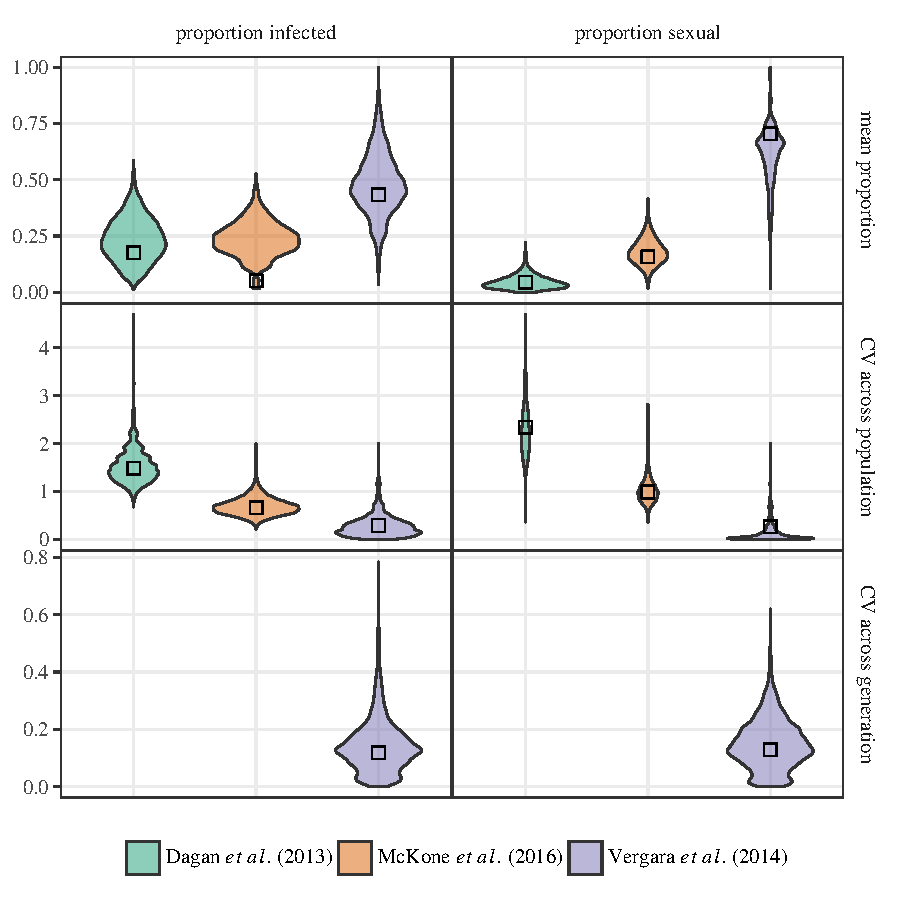
\includegraphics[width=\textwidth]{../fig/smc_summary.pdf}
\caption{{\bf Summary statistics of the observed data vs. distribution of summary statistics of the simulated data from the posterior samples.}
Dotted horizontal line represents observed summary statistics.
Violin plots show weighted distribution of fitted summary statistics (i.e., summary statistics that were accepted during Approximate Bayesian Computation). 
Error bars show 95\% weighted quantiles of predicted summary statistics.
For each posterior sample, 10 simulations are run and each simulated system is sampled at random 100 times so that each sample consists of equal number of populations as number of sites in fitted data. 
Then, summary statistics are calculated for each sample and are weighted by their corresponding weights.
}
\label{fig:smcsumm}
\end{figure}

To further diagnose the fit, we compare the predicted relationships between mean infection prevalence and mean frequency of sexual hosts in each population (averaged over last 100 generations) with the observed data (\fref{ivs}).
Note that \fref{ivs} appears to be more variable than \fref{smcsumm} as it plots density of all simulated populations and hence accounts for uncertainty in unsampled populations.
Despite being able to reproduce the summary statistics reported by \cite{dagan2013clonal} well, 
our model is unable to capture the qualitative trend between proportion of sexual hosts and proportion of infected hosts (\fref{ivs}; \cite{dagan2013clonal}).
Both simulated data and observed data mostly consist of asexual populations
but our model predicts sexual reproduction to be maintained when infection prevalence is high ($> 40\%$). 
On the other hand, \cite{dagan2013clonal} data suggests that sexual reproduction is only maintained when infection prevalence is low ($< 20\%$).
Similarly, overestimation of infection prevalence is strongly pronounced in our prediction of system studied by \cite{mckone2016fine}.

While there are a few data points that appear to be outliers compared to our predictions for \cite{vergara2014infection},
it is important to note that \fref{ivs} does not capture temporal variation as we average over 100 generations to obtain the ``mean'' relationship.
The observed data are more likely to be samples across a few generations and the cyclic nature of the Red Queen dynamics is likely to have created more variation in the data.
On the other hand, \cite{vergara2014infection} reported greater than 90\% sexual snails throughout 5 years in one of their study sites but it seems unusually high based on our model prediction.

\begin{figure}[!ht]
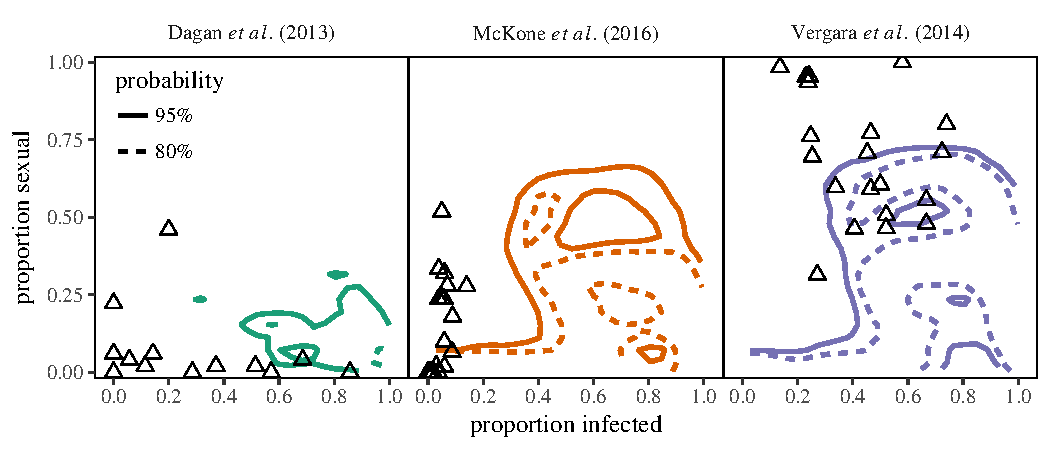
\includegraphics[width=\textwidth]{../fig/simulated_data.pdf}
\caption{{\bf Predicted relationship between mean infection prevalence and mean proportion of sexual hosts in each population.}
For each posterior sample, 10 simulations are run.
For each population within a simulation, mean infection prevalence and mean proportion of sexual hosts is calculated by averaging across last 100 generations. 
Each population is assigned equal weight as the parameter that simulated the population.
Colored contour lines show 95\% weighted highest posterior density region.
Open triangles represent observed data; proportion of sexual hosts is computed from proportion of male hosts.
Open circles represent observed mean proportions averaged across years. Dotted lines around open circles represent ranges of proportion of sexual and infected hosts observed in each site.
}
\label{fig:ivs}
\end{figure}

We find that there is a region (around 30\% infection prevalence) in which proportion of infected hosts remains almost constant while proportion of sexual hosts increases (most clearly visible in the fits to \cite{mckone2016fine} and \cite{vergara2014infection}).
As transmission rate ($\beta$) increases, selection for sexual hosts increases but increasing number of resistant offsprings prevents further infection from occuring and can decrease overall infection prevalence.
Such a trend is consistent with previous results by \cite{lively2001trematode} who noted that there is a region in which both sexual and asexual reproduction can be selected exclusively under same infection prevalence.
We also find that proportion of sexual hosts decreases when infection prevalence is very high.
Decrease in fitness of sexual hosts associated with increase in prevalence was predicted by \cite{ashby2015diversity}; 
it can also be found in an earlier work by \cite{lively2010epidemiological} although it was not discussed in the paper.

\subsection*{Not edited:}



Parameter estimates for \cite{vergara2014infection} are presented in \fref{smcparam}.
The most surprising result is that the posterior distributions of the scale parameter for cost of sex, $c_b$, is much wider than the prior distribution and have noticeably higher mean: (mean (95\% credible interval)) 1.30 (0.80-1.97).
\cite{ashby2015diversity} defined $c_b$ as additional costs and benefits of sex, where $c_b=1$ corresponds the two fold cost.
Under their interpretation, our estimate corresponds to the following mean and 95\% CIs for cost of sex: 1.54 (1.02-2.50).
Note that some posterior samples range $c_b > 2$, corresponding to faster growth rate of sexual hosts than asexual hosts.
Simulated data from these posterior samples mostly consist of populations with almost 100\% sexual hosts.
While these estimates are not entirely impossible given that \cite{vergara2014infection} observed almost 100\% sexual snails in one of their sampling sites throughout 5 years, their observation is likely to be a sampling artifact since an earlier work sampled at the same site reported much lower frequency of sexual snails \citep{vergara2013geographic}. %% TODO: double check sources

\begin{figure}[!ht]
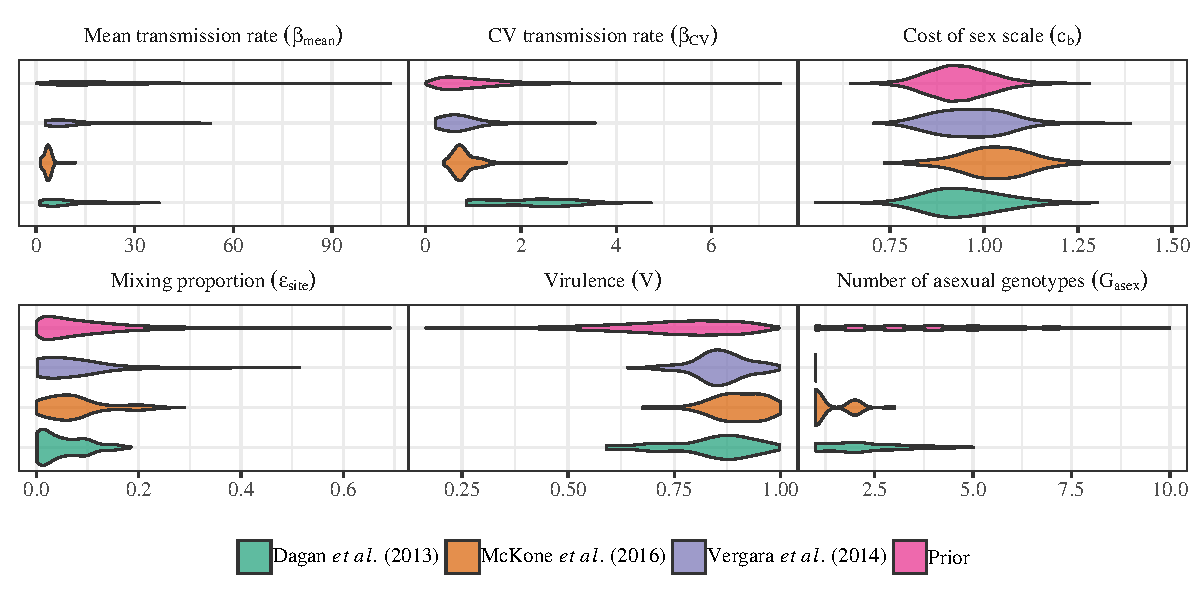
\includegraphics[width=\textwidth]{../fig/posterior.pdf}
\caption{{\bf Parameter estimates from Sequential Monte Carlo Approximate Bayesian Computation.}
Lines repreesnt 95\% quantile and points represent mean posterior estimates. 100 posterior samples were obtained from SMC ABC. Prior distributions are specified in [TODO].
}
\label{fig:smcparam}
\end{figure}

The model estimates high virulence overall: (mean (95\% CI)) 87.0\% (67.5\%-98.7\%).
In contrast to \cite{lively2010epidemiological}, who modeled 1 asexual genotype competing with 9 sexual genotypes, our model estimate shows that higher asexual to sexual genotypic ratio can be supported ($G_{\textrm{\tiny asex}}$ panel in \fref{ivs}).
274 out of 300 posterior samples estimate $G_{\textrm{\tiny asex}} = 1$; 25 samples estimate $G_{\textrm{\tiny asex}} = 2$; and 1 sample estimates $G_{\textrm{\tiny asex}} = 3$.
However, we find that it is still necessary for sexual hosts to have higher genetic diversity than asexual hosts.

Finally, a power analysis show that the power for detecting a positive correlation between infection prevalence and frequency of sexual hosts in \cite{vergara2014infection} population is almost 0 (\fref{power}).
We find that there is much higher (but still low) power to detect a negative correlation.
Increasing number of samples per site has small effect on power once the sample size greater than 50.
Increasing number of sites leads to greater increase in power but the power appears to saturate as number of sites increases.

\begin{figure}[!ht]
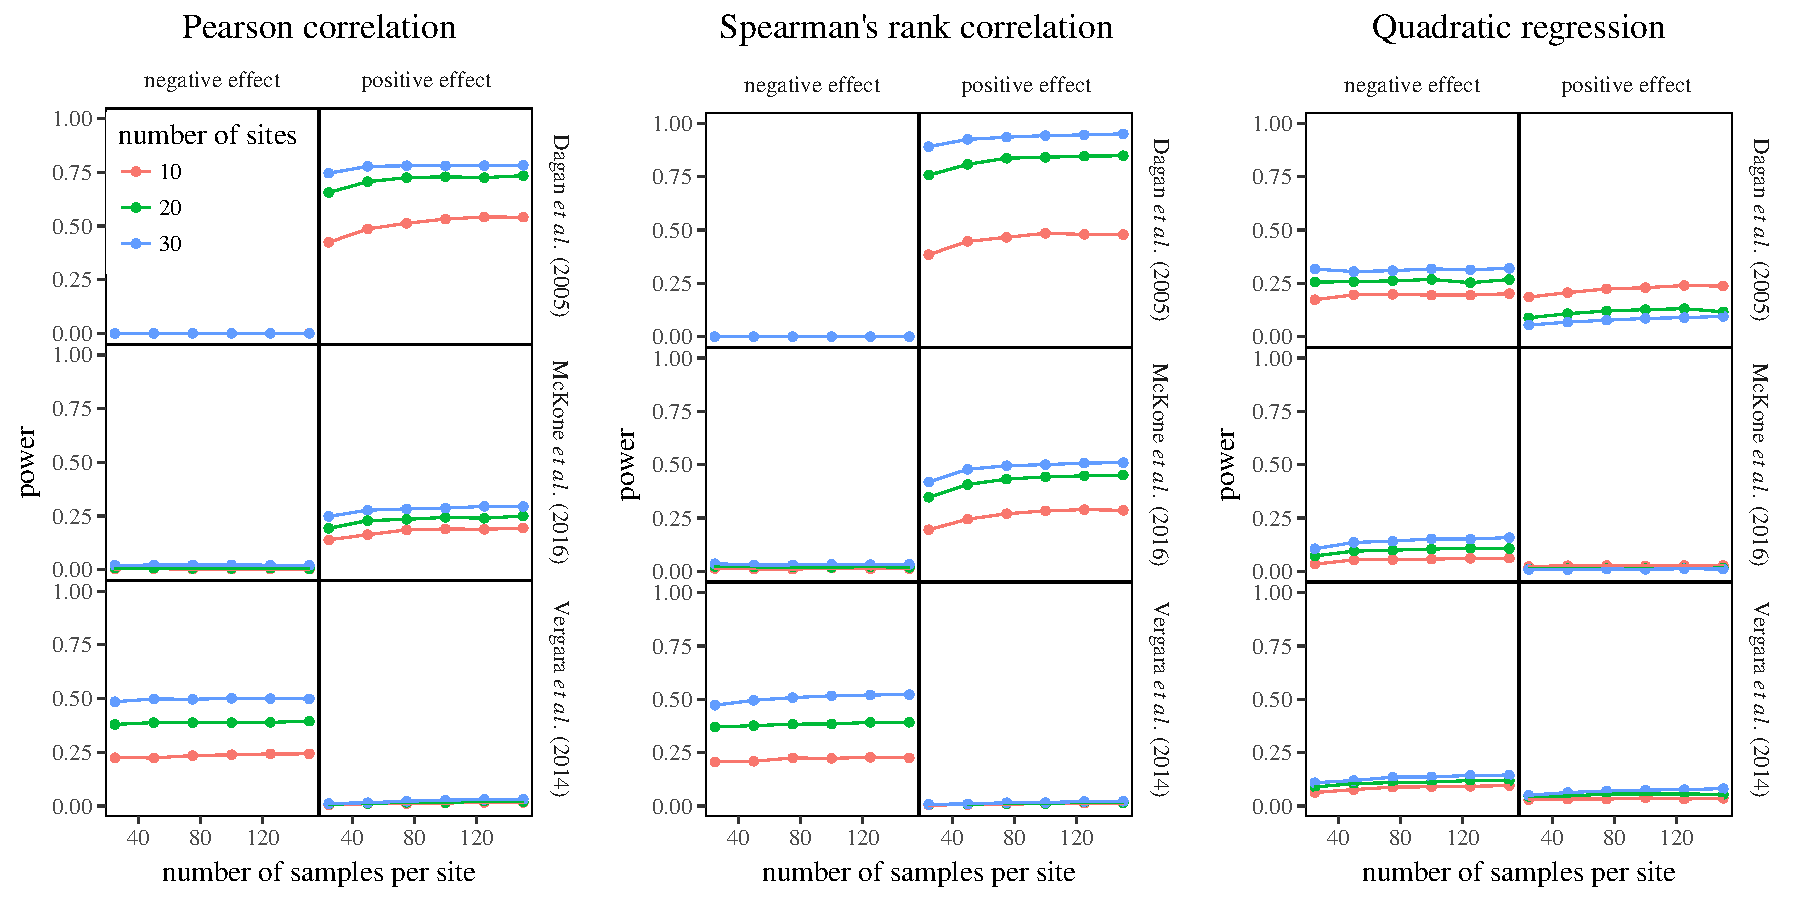
\includegraphics[width=\textwidth]{../fig/power.pdf}
\caption{{\bf Power to detect a statistically clear correlation between infection prevalence and frequency of sexual hosts.}
(a) Power to detect a positive correlation. 
(b) Power to detect a negative correlation. 
(c) (Contour) power to detect a positive correlation as a function of transmission rate parameters and (points) marginal posterior distributions.
Spearman's rank correlation was used to test for correlation between infection prevalence and frequency of sexual hosts in simulated data from the posterior distributions.
Contour plot is created by taking the mean posterior estimates and assuming 20 sites and 100 samples per site.
}
\label{fig:power}
\end{figure}

\section{Discussion}

Our results challenge ways in which the Red Queen Hypothesis for sex has been studied.
Previous modeling studies have either relied on assumed parameters [CITE] or explored parameter spaces [CITE]
to understand sexual reproduction maintained by host parasite coevolution.
Here, we show that (1) model parameters are estimable and (2) a simple Red Queen model with population structure can reproduce key summary statistics observed across three different snail systems (\fref{smcsumm}).
While our model is able to reprouce observed summary statistics, there still remain some discrepancies between model prediction and observed relationship between infection prevalence and frequency of sexual hosts across populations.
These discrepancies suggest a simple host-parasite model is not sufficient to explain sexual reproduction observed in nature.
% We also find that detecting a positive correlation between infection prevalence and frequency of sexual hosts is difficult (\fref{power}) and hence not a good measure for measuring the effects of the Red Queen.

A model that does not fit well can sometimes tell us more about the system of interest than a model that fits well.
For example, there is a clear mismatch between the model and the data presented by \cite{dagan2013clonal} (\fref{ivs}).
The snail populations studied by \cite{dagan2013clonal} live in intrinsically different environments from two other snail populations that we consider.
For example, some habitats are subject to seasonal flash floods, which can affect reproductive strategies of snails \citep{ben2007temporal}.
Althuogh we cannot estimate the strength of the effect of environment on sexual reproduction of snails relative to that of the effect of parasites, it is likely to be a cause of the bad fit.
We conclude that the Red Queen Hypothesis alone cannot explain maintenance of sexual reproduction in this population.

The only system that our model could resemble fairly well is one studied by \cite{vergara2014infection}.
In order for our model to produce similar summary statistics as those observed in nature, it requires the scale parameter ($c_b$) for the cost of sex to have mean greater than 1 (\fref{smcparam}).
A model that assumes two fold cost of sex ($c_b=1$) would not have fitted well.
However, from an inferential point of view, $c_b > 1$ does not necessarily imply that cost of sex is less than two fold.
We interpret an estimate of $c_b > 1$ as amount of compensation required in order for the model to reproduce observed data.
Additional compensation can include less than two fold cost of sex or any other mechanisms that can promote sex.

A suitable candidate for model compensation is increase in host genetic diversity.
Although exact genetic architecture that determines trematode infecion in snails (e.g., loci involved in parasite resistance) is not known {CITE}, genetic diversity of snails that have been documented is far greater than what we have assumed \citep{king2011parasites, dagan2013clonal}.
In addition, increasing genetic diversity of the model may resolve overestimation of infection prevalence (\fref{smcsumm}).
Previous studies have shown that moderately high genetic diversity can allow sexual hosts to escape infection more easily and therefore reduce prevalence of infection given similar amount of sexual reproduction \citep{lively2010effect, king2012does, ashby2015diversity}.
Overall, our results indicate that more modeling effort is required to understand prevalence of sexual reproduction in nature.

Our power analysis (\fref{power}) constrasts with the positive correlation predicted by \cite{lively1992parthenogenesis, lively2001trematode} and findings of many empirical studies that have confirmed the prediction \citep{lively1987evidence, lively2002temporal, kumpulainen2004parasites, vergara2013geographic, mckone2016fine}.
The power analysis predicts almost no power for detecting a positive corrleation in the population studied by \cite{vergara2014infection} and relatively higher but still low power for detecting a negative correlation.
This result may appear to contradict an earlier work by \cite{vergara2013geographic} that reported a positive correlation between between infection prevalence and male frequency in the same lake but there is a simple explanation for the difference.
The key premise behind the postive correlation predicted by \cite{lively2001trematode} is that there must be large variation in infection prevalence.
In particular, range of prevalnece must be wide enough so that the sample includes sites with almost no infected hosts (hence no sexual hosts) and those with reasonably high proportion of infected hosts to maintain sexual reproduction through parasitism \citep{lively2001trematode}.
Since all four habitats studied by \cite{vergara2014infection} consists of populations with high prevalence and high frequency of sexually reproducing hosts, positive correlation vanishes.
Instead, studying a system with larger variation and lower mean prevalence will yield much high power (\fref{power}(c)).

% While predicting a positive correlation between prevalence of infection and frequency of sexual hosts, \cite{lively2001trematode} also noted that there is a region at which expected infection prevalence overlaps between sexual and asexual populations. 
% Within this region lies the association between increase in sexual reproduction and decrease in infection prevalence observed in \fref{ivs}.
On the other hand, negative correlation between prevalence of infection and frequency of sexual hosts can be explained by cycling of host and parasite populations.
A main component of the Red Queen Hypothesis is that negative frequency dependence drives oscillation in both host and parasite population \citep{hamilton1980sex}.
When temporal variation is taken into account, association between infection prevalence and frequency of sexual hosts can change depending on what phase each of the sample population is going through in its cycle (\fref{cycle}).
The negative correlation in the population does not contradict the positive correlation predicted by \cite{lively2001trematode} because their prediction did not take temporal variation into account.

\begin{figure}[!ht]
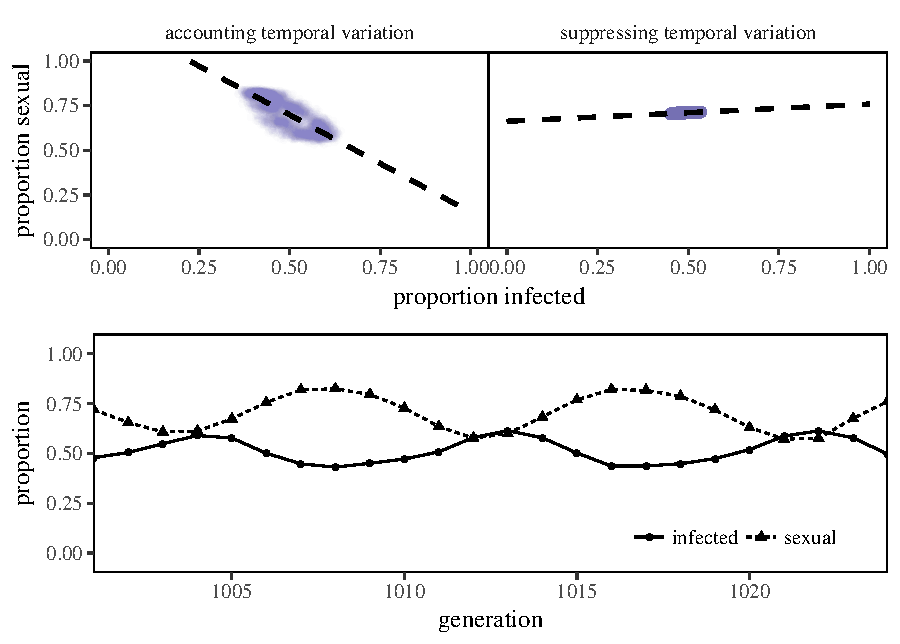
\includegraphics[width=\textwidth]{../fig/cycle_example.pdf}
\caption{{\bf Simulated data from the posterior distribution fitted to \cite{vergara2014infection}.}
A particular simulation is chosen from the posterior distributions to demonstrate that it is possible to predict opposite relationship when temporal variation is taken into account. (Top left) each point represents proportion of infected hosts and proportion of sexually reproducing hosts of each population at each generation. Last hundred generations are plotted. (Top right) each point represents mean proporiton of infected hosts and mean proportion of sexually reproducing hosts of each population averaged over the last hundred generations. Dashed lines represent least squares fit to all point. (Bottom) A typical host parasite cycle observed in a population from this simulated data. %% TODO: need to report parameter values?
}
\label{fig:cycle}
\end{figure}

%% still thinking about conclusion

\bibliography{redqueen}
\end{document}
